\section{Demonstrator Prototype}
\label{sec:prototype}

To construct a representative demonstrator prototype illustrating the use of Node.js, we developed a web application inspired from the Java EE project. By building the project from the bottom with Node.js using MongoDB and Express as tools, we developed a portal based on art commerce. The web application for auctioning artworks was constructed as a prototype to demonstrate the substantial assets and benefits of Node.js. Both back-end and front-end are implemented in JavaScript. 

\subsection{Prototype}
As mentioned, the prototype is inspired by the Java EE project with focus on artworks instead of products. Our main focus for this prototype (because of time constraints) was to implement the most essential features to make the application work as intended.
\\\\
The entities Artwork and Account are quite similar. Viewing accounts and arts in the application has the same layout. Creating an account and submitting an artwork are also similar with the exception of uploading an image when submitting an artwork, and therefore only showing images of functionalities for entity Artwork.

\begin{figure}[h!]
  \centering
  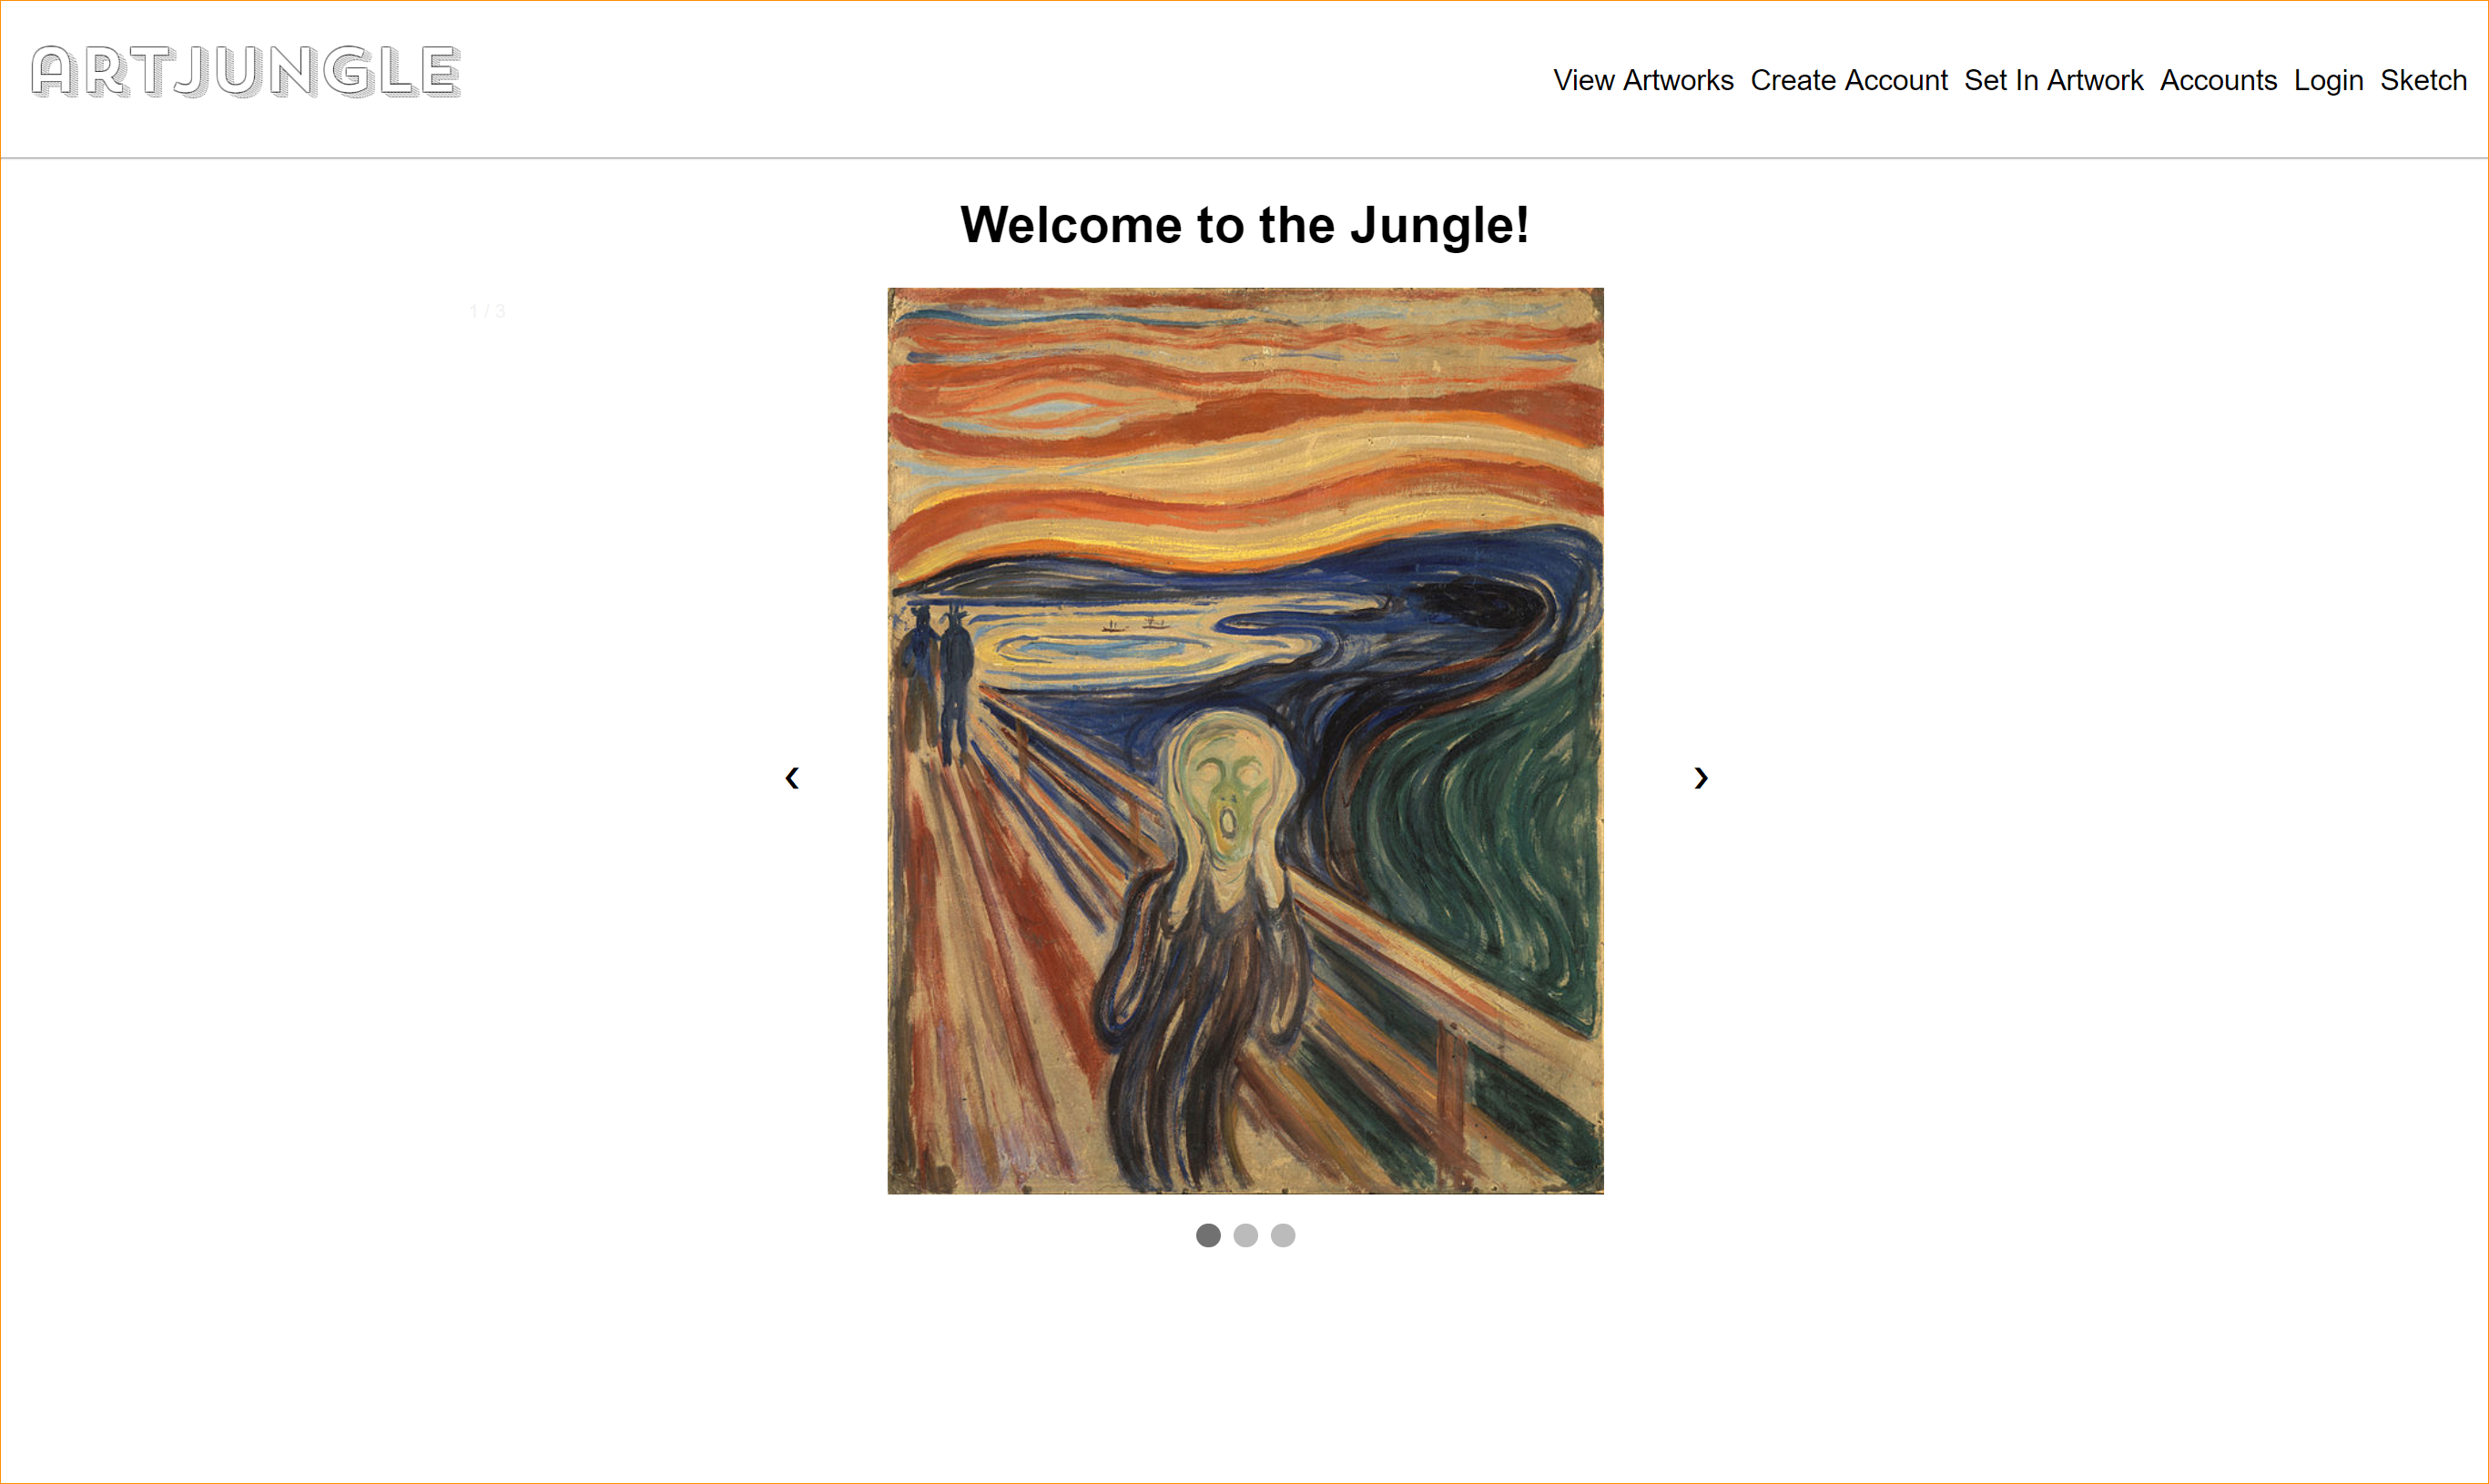
\includegraphics[scale=0.3]{figs/homescreen.png}
  \caption{Homescreen of the application}
\end{figure}

The home screen, as shown in figure 4, is very simple. The user will be met with a slideshow over some of the arts being available for auction. The user can also at any time navigate to other sites by clicking on a link in the header of the page. 

\begin{figure}[h!]
  \centering
  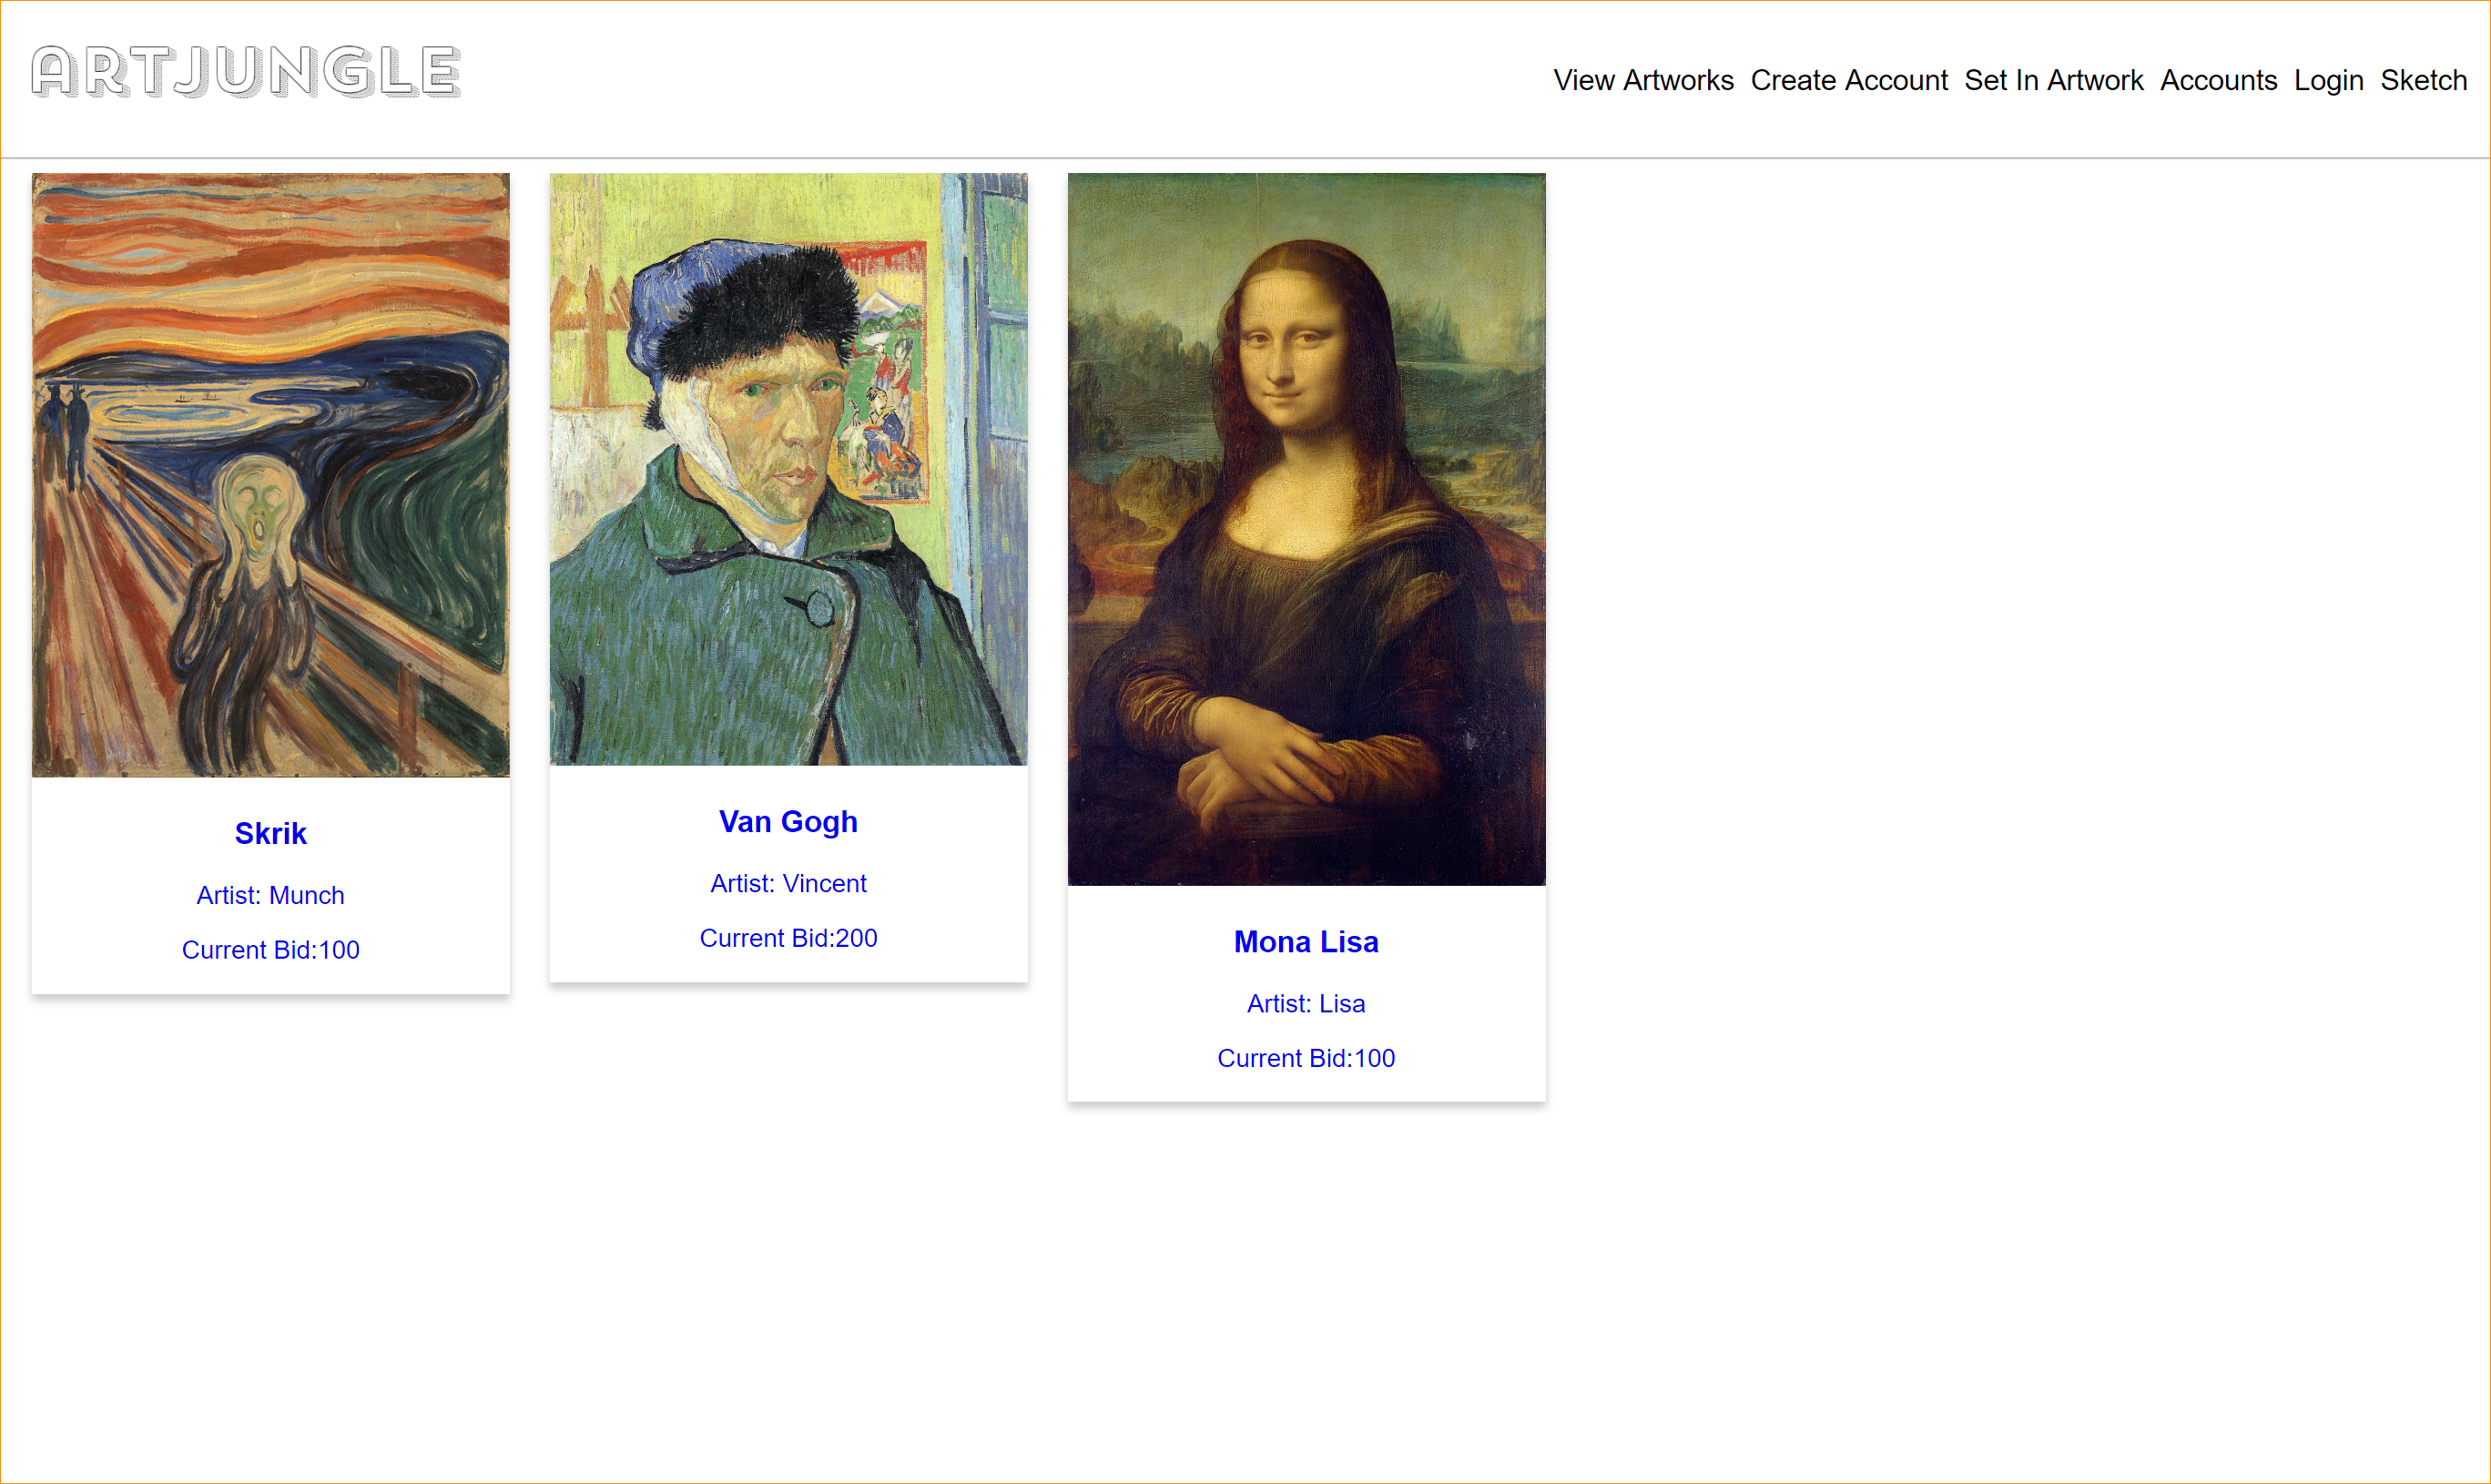
\includegraphics[scale=0.3]{figs/viewartworks.png}
  \caption{Overview of artworks}
\end{figure}

When navigating to "View Artworks", the user will see an overview of the artworks, as shown in figure 5. The user will be able to click on an artwork to get more details about that particular artwork. 

\begin{figure}[h!]
  \centering
  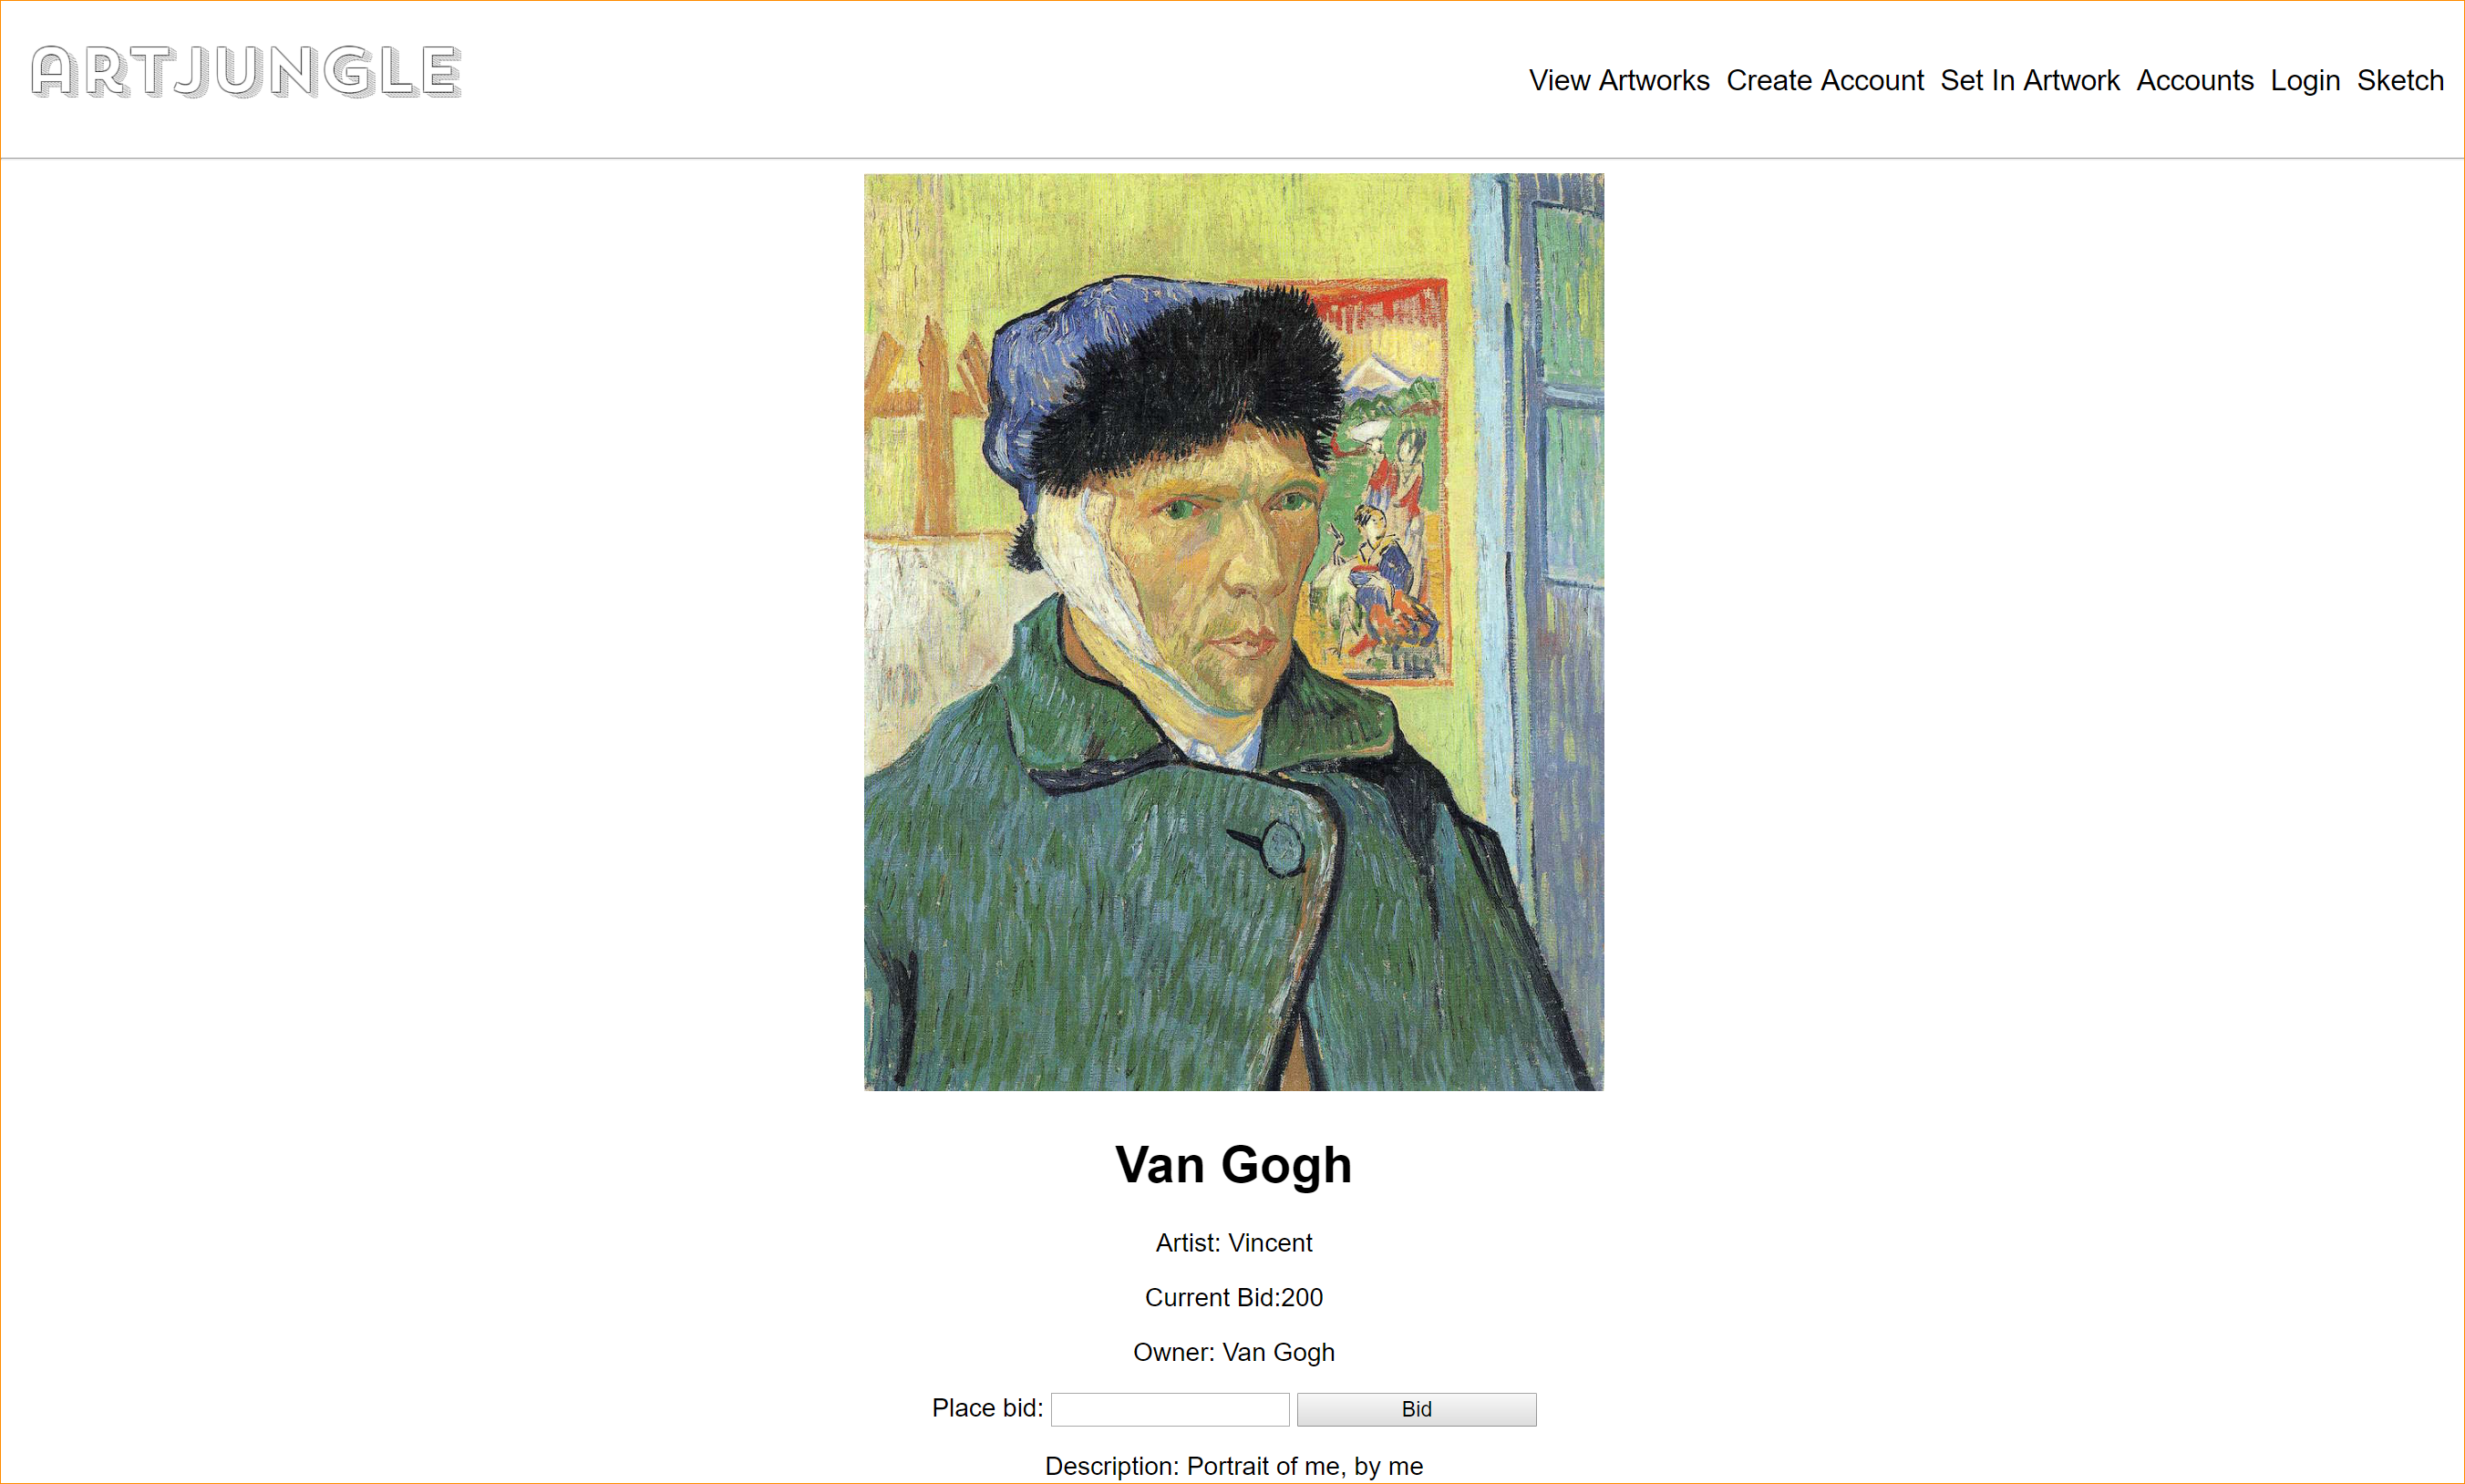
\includegraphics[scale=0.3]{figs/artwork.png}
  \caption{Details about an artwork}
\end{figure}

After clicking on an artwork, the user will see more details about the artwork, as shown in figure 6. The user will be able to bid on the artwork, and after a bid is made, the bid will be updated.  

\newpage
\begin{figure}[h!]
  \centering
  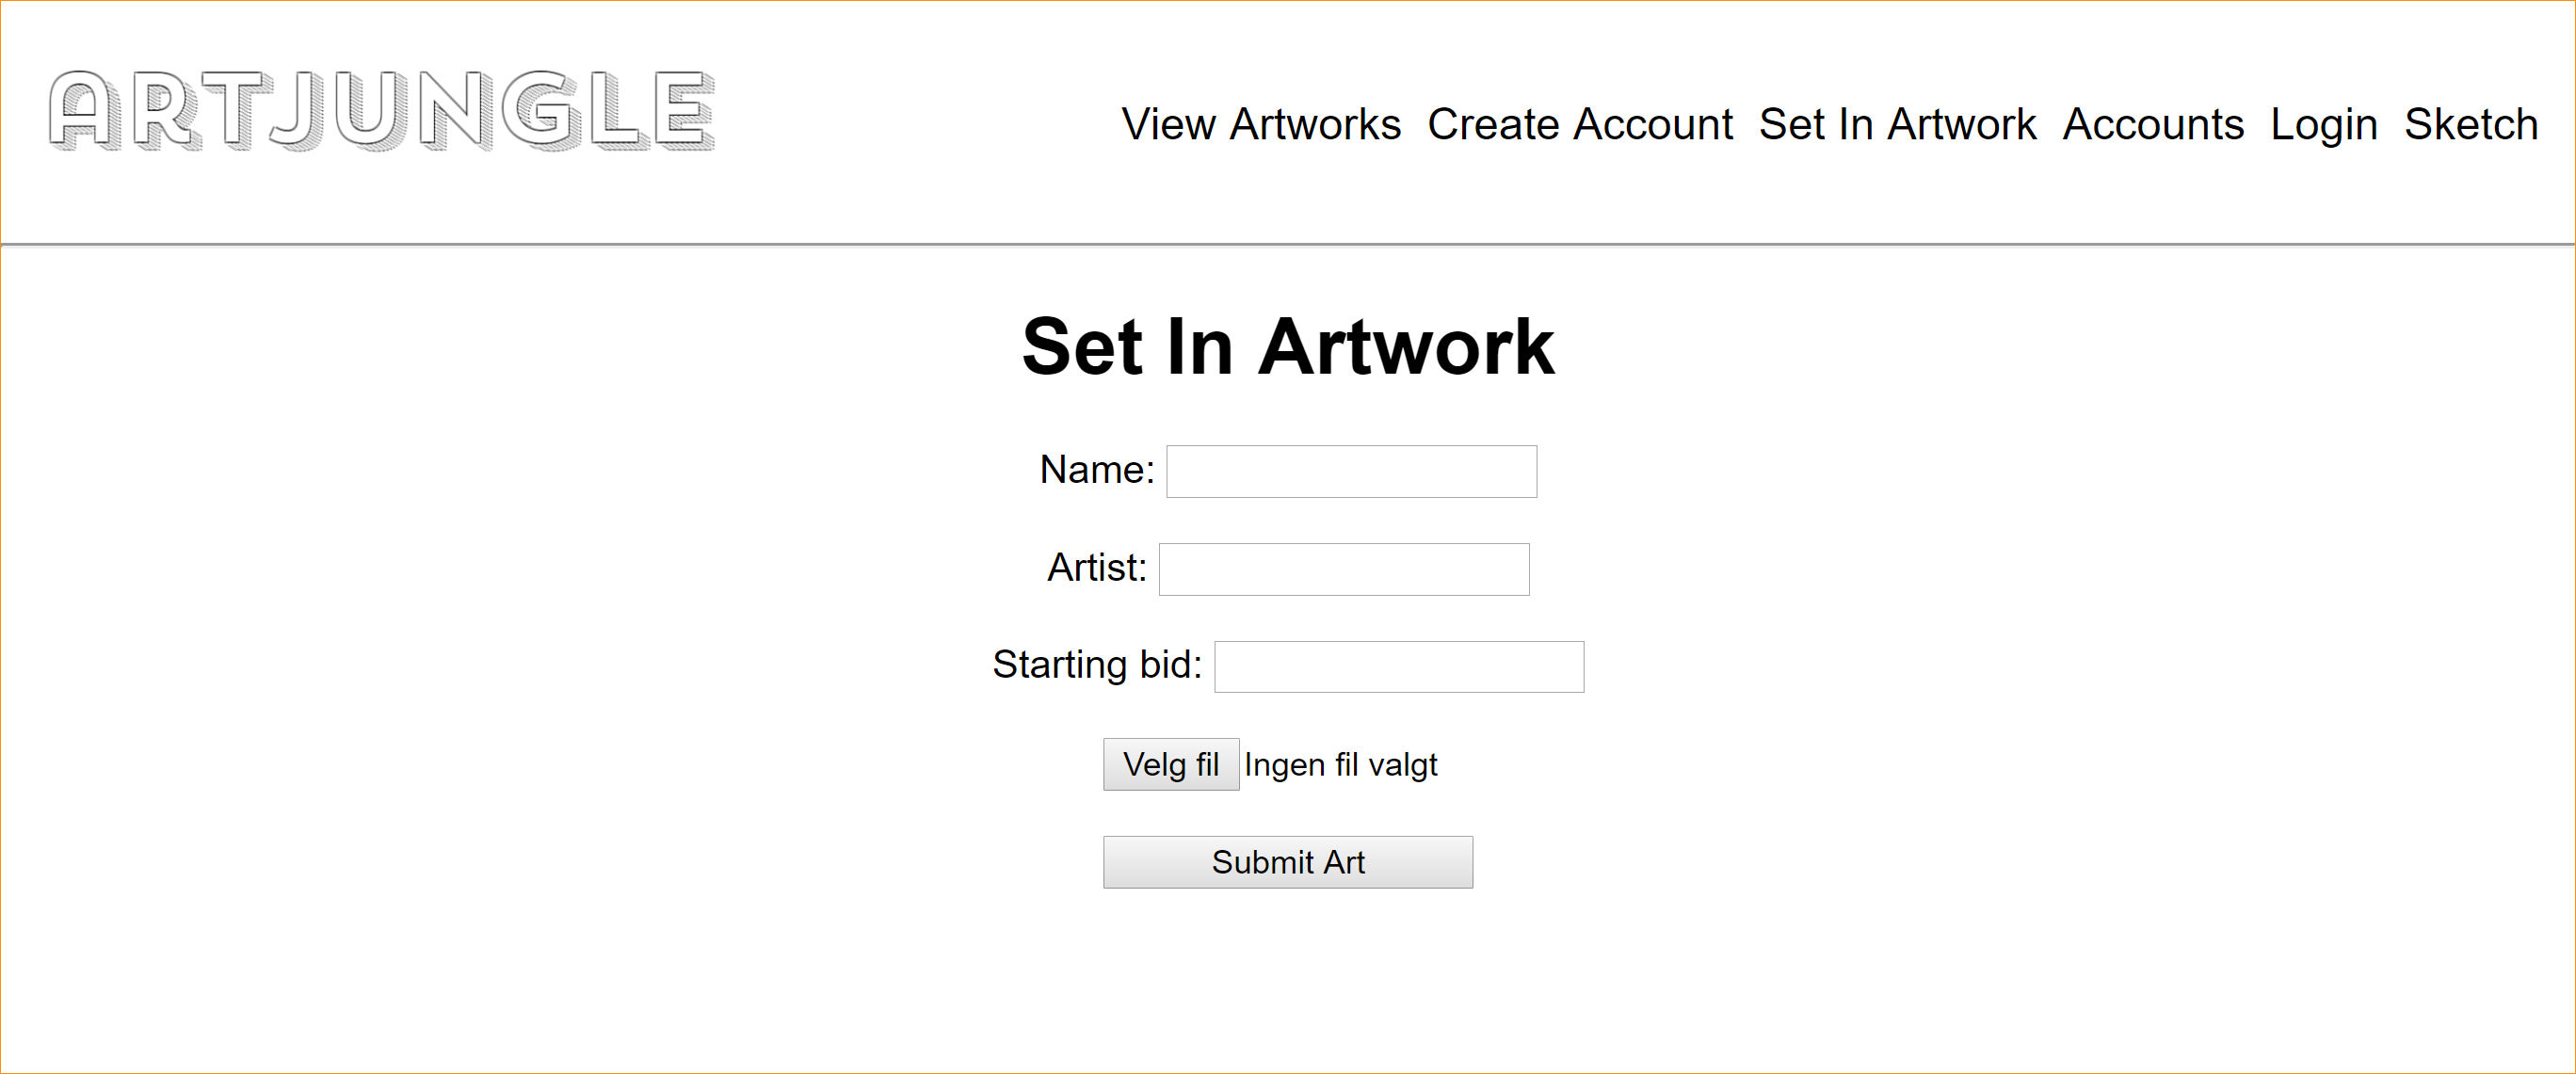
\includegraphics[scale=0.3]{figs/submitartwork.png}
  \caption{Submit an artwork}
\end{figure}

The user will be able to submit artworks by filling a form and adding an image of the artwork by clicking on "Set in Artwork", shown in figure 7. 

\begin{figure}[h!]
  \centering
  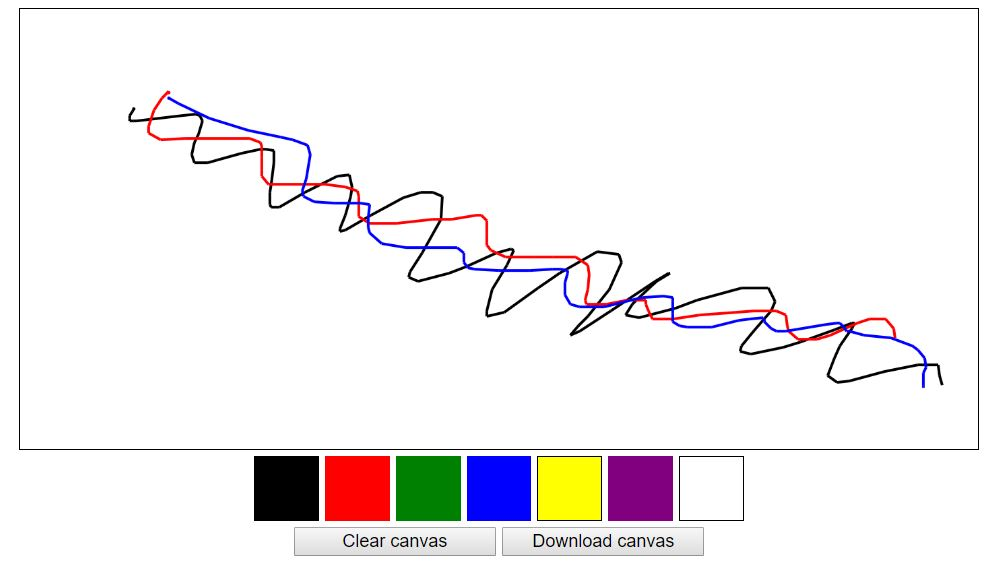
\includegraphics[scale=0.5]{figs/sketchApp.JPG}
  \caption{Details about an artwork}
\end{figure}

Lastly, the figure 8 shows that the user is able to draw on a canvas. The user can choose between multiple colors, clear the canvas or download the drawn image. With the module Socket.io, multiple users are able to draw on the same canvas at the same time. More details about this module will be mentioned later.

\subsection{The package.json}
The requirement of Node.js applications is the package.json file which contains several properties. Some of the crucial properties containing in the package.json file are name (name of the application), version, description (description of the application) and main (which points to the entry point of the application). The file also contains scripts (which will run when we need to perform repetitive tasks), author name, licence and dependencies. The properties summarize a representation of the Node.js application. 
\newline \newline
Listed below is our dependencies from \textbf{\textit{package.json}} used in our Node.js application.
\begin{minted}{json}
{
  ...
  "dependencies": {
    "bcrypt": "^1.0.3",
    "body-parser": "^1.18.3",
    "canvas2image": "^1.0.5",
    "ejs": "^2.6.1",
    "express": "^4.16.4",
    "express-fileupload": "^1.0.0",
    "formidable": "^1.2.1",
    "fs": "0.0.1-security",
    "mongodb": "^3.1.8",
    "mongoose": "^5.3.7",
    "morgan": "^1.9.1",
    "nodemon": "^1.18.6",
    "socket.io": "^2.1.1"
  }
}
\end{minted}
The dependencies are a requirement for the application. The modules must be installed to be able to run the prototype on another computer with Node.js, but can simply be installed with "npm install". 
\subsection{Architecture and implementation}
The architectural style is based on the MVC pattern. The Model-View-Controller Pattern defines the separation of the interconnected parts of our application. This is a commonly used framework of developing web applications. \cite{chrome:MVC}
\newline\newline
\textbf{Model}
\newline
Contains a representation of an object and also the logic to update the controller when data changes. The structure in this part covers Mongoose, which is a tool for MongoDB object modeling that works in an asynchronous environment. By using this tool we created a connection with MongoDB and defined our model through the Schema interface. Below we included code from the file \textbf{\textit{account.model.js}} to represent the structure of the account object.
\begin{minted}{JavaScript}
const AccountSchema = mongoose.Schema({
    name: String,
    phone: String,
    email: String,
    password: String,
    photo: String,
    bids: [{
        type: mongoose.Schema.Types.ObjectId,
        ref: 'Bid'
    }],
    artworks: [{
        type: mongoose.Schema.Types.ObjectId,
        ref: 'Artwork'
    }]
}, {
    timestamps: true
});
\end{minted}
Since MongoDB is a NoSQL database, there is not actual relation between the different entities in the model. But since we are using mongoose, we can just add the different entities like we did in the example above. This will save the id's of the relational entities, which can later be populated (see controller).
\\\\
\textbf{View}
\\
The view is the implementation and visualization of the data which the model includes. In this section we used Embedded JavaScript (EJS), which is a flexible template engine suited for Node.js. With EJS we can directly render pages dynamically with Express. Using EJS was simple, readable and convenient for the MVC structure. EJS makes it so that one can use functions such as .foreach() combined with the HTML code to avoid code repetition, as shown below from \textbf{\textit{view\_account.ejs}}.

\begin{minted}{HTML}
<% account.forEach(function(account) { %>
<div class="card">
    <a href="accounts/<%= account.id%>">
        <img src="<%= account.photo %>" style="width:100%; height:50%">
        <div class="container">
        
            <h3><%= account.name %></h3>
            <p>Phone: <%= account.phone %></p>
            <p>Email: <%= account.email %></p>
        </div>
    </a>
</div>
<% }); %>
\end{minted}
Here we get the account information in JSON-format from the backend, and use the .foreach() function to loop through each one and create the "cards" showing all the information for each account.
\\\\
\textbf{Controller}
\\
Separates the view and model while acting on both, by controlling the flow into model object when updating the view of the changed data. Here we created the REST API for our application. Here is an example from of the findAll() function from \textbf{\textit{account.controller.js}}.

\begin{minted}{JavaScript}
exports.findAll = (req, res) => {
    Account.find()
    .populate('bids')
    .populate('artworks')
    .then(account => {
        res.render('pages/view_accounts',{
            account:account
        })
    }).catch(err => {
        res.status(500).send({
            message: err.message || "Some error occurred while retrieving account."
        });
    });
};
\end{minted}
This is an event-handler for the REST API of our application. The function findAll() takes a request and response (req,res) as parameters, finds the requested accounts, populates the objects with data for the relations (see model), and sends the accounts back as a response (and renders the redirected page, this is ejs specific). If Account.find() returns an error, the error will be caught and an appropriate status code and message will be sent.
\\\\
We also attempted to create log-in functionality for the application, but we did not have the time to actually add functionalities like sessions and roles. We have added a password (which is hashed in the database) and log-in page to authenticate a user, but this has no actual purpose. 

\subsection{Development experience and Java EE comparison}
Setting up the the database and server for this prototype was a breeze compared to setting up the server and database in Eclipse when we created the Java EE application. It has also been much more stable for us, which has resulted in better flow in the development of the prototype. Also small things like restarting the GlassFish server in Eclipse was very slow, while the Express server in our prototype starts instantly (and automatically once we started using a package called nodemon), which made for a much better experience when developing the application.
\\\\
We also have some previous experience with JavaScript/TypeScript, and getting into the code in Node.js did not require much time and resource. We started with some simple tutorials for setting up the skeleton of the application with REST in an MVC architecture and developed from there. Harder tasks like asynchronous functions and callbacks also became manageable very quickly.
\\\\
Coding in Node.js and Java EE was actually pretty similar. Our biggest issues with developing the Java EE was not only code related, but rather the configurations and unstable server/database. We have a lot of experience with Java SE from before, so writing the code in Java EE was pretty simple (except new things like annotations and relations between entities) and the structure of the application was mostly straight forward. To compare the two here is a short codesnippet from the GET-request in the REST-API from each of the applications.
\\\\
Node.js:
\begin{minted}{JavaScript}
module.exports = (app) => {
  const artwork = require('../controllers/artwork.controller.js');
   app.get('/artworks', artwork.findAll);
   
   app.get('/artworks/:artworkId', artwork.findOne);
...
}
\end{minted}
Java EE:
\begin{minted}{Java}
...
@GET
@Path("/products")
@Produces({MediaType.APPLICATION_XML, MediaType.APPLICATION_JSON})
public Products getProducts() {
	return dao.getAllProducts();
}

@GET
@Path("/products/{id}")
public Response getProduct(@PathParam("id") String id) {
	Product product = dao.getProduct(id);
	if (product == null)
		throw new NotFoundException();
	return Response.ok(product).build();
}
...
\end{minted}
Both of these code snippets are methods/functions that basically do the same thing. They route a request to the business logic, where the data is retrieved from the database and is responded back. The difficulty of understanding the code here is pretty similar, but one can see that there is a big difference in the amount of code written, 5 lines for Node.js and 15 for Java EE (3x as many lines). This is mostly because of the method structure and annotations, whereas Node.js, which uses a listener (app), can handle the requests themselves in just one line each.
\\\\
Looking into a more quantitative comparison we can compare the total amount of lines of code.  Not taking into account such as dependencies, packages, tests and config files, we end up around 900 lines of code for Node.js project, and about 2300 lines for the Java EE. This makes sense since most of the code for Node.js is simpler, less structured and not as strongly typed, which makes it shorter. The Node.js prototype is also not as complex as the Java EE application. The Java EE application has multiple services, more entities and also a bit more functionality, so we have to take that into account. 
\\\\
If we look at the size on disk of the two projects though, we find something interesting. The Node.js project is taking up about 26.2 MB of space on disk (not counting .jpg files), whereas the entire Java EE project only takes up about 276 KB. This is mostly because of the nodemodules folder, that contains all the packages used, which takes up 26.1 MB of the 26.2 MB used. This leaves about 100KB of space for the rest of the files, which gives a more sensible code-to-diskspace ratio compared to the Java EE project. But one can see that because of Node.js projects have to save packages locally, it is not nearly as efficient as Java EE at using disc space.
\\\\
Our experience with developing a prototype using node.js has been good. Node.js was very simple to use, which one can tell by the progress we made with the prototype (compared to the Java EE application), and also at the amount of code written over this time period. Though it is lacking some robustness, security and structure compared to the Java EE application, it has been more stable, just as powerful and easier to make.